\documentclass{article}
\usepackage{titling}
\usepackage{lipsum}
\usepackage{amsmath}
\usepackage{listings}
\usepackage{graphicx}
\usepackage{subcaption}
\usepackage{pgfplots}
\usepgfplotslibrary{statistics}



\begin{document}
\noindent
\begin{minipage}[t]{0.6\textwidth}
    \begin{flushleft}
        \LARGE\textbf{Math 343 - Homework 2} \\
        \vspace{6pt} % add 6pt of vertical space
        \hrule width 10cm
        \vspace{12pt}
        \large\textbf{Preston Duffield} \\
        \large Western Washington University \\
        % \today
        April 14, 2023
        \vspace{24pt}
    \end{flushleft}
\end{minipage}

\section*{Question 1}

Data with a rightward skew would produce a normal probability plot with a positive curvature.
Below is an example of a histogram that would produce a positively curved normal probability plot. \\


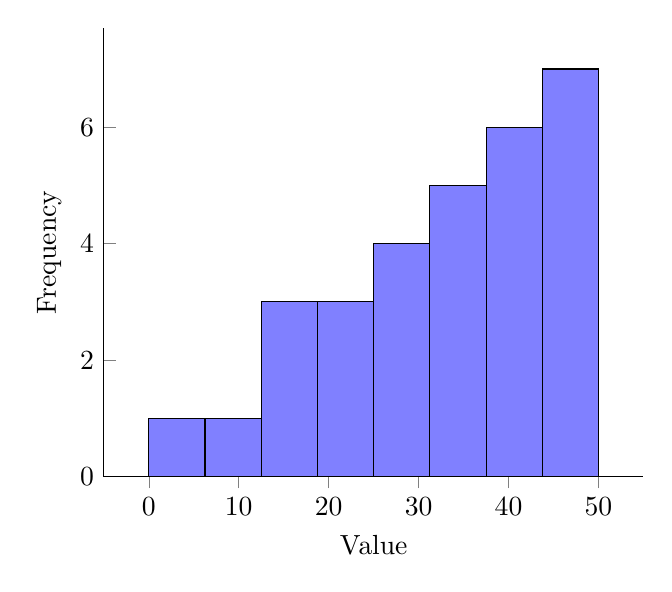
\begin{tikzpicture}
  \begin{axis}[
      ybar,
      ylabel={Frequency},
      xlabel={Value},
      ymin=0,
      axis lines*=left,
      % xtick=data,
      % nodes near coords,
      % nodes near coords align={vertical},
  ]
  \addplot[
      fill=blue!50,
      hist={
          bins=8,
          data min=0,
          data max=50,
      },
  ] table[row sep=\\,y index=0] {
      data \\
      36 \\ 30 \\ 25 \\ 40 \\ 20 \\ 6 \\
      35 \\ 9 \\ 50 \\ 24 \\ 40 \\
      15 \\ 16 \\ 17 \\ 50 \\ 21 \\
      25 \\ 50 \\ 40 \\ 30 \\ 32 \\
      35 \\ 36 \\ 38 \\ 40 \\ 42 \\
      45 \\ 46 \\ 48 \\ 50 \\
  };
  \end{axis}
  \end{tikzpicture}
\clearpage
\section*{Question 2}

\section*{Question 3}

\subsection*{a)}
\begin{figure}[h]
    \centering
    \includegraphics[width=0.5\textwidth]{./images/3_a.png}
    \caption{The output of the test for two variances from Minitab.}
    \label{fig:3_a}
  \end{figure}
  Since the P-value $> \alpha$ we can conclude the following. There is enough statistical evidence to support the hypothesis that both of the variances are equal.

\subsection*{b)}
\begin{figure}[h]
    \centering
    \includegraphics[width=0.5\textwidth]{./images/3_b.png}
    \caption{The output of the two sample t test from Minitab. Assuming equal variances.}
    \label{fig:3_a}
  \end{figure}
  Since the P-value $= 0.962 > \alpha$ we can conclude the following. There is enogh statistical evidence to support the hypothesis that the two means are equal.
\subsection*{c)}

\begin{figure}[h]
    \centering
    \begin{subfigure}[b]{0.4\textwidth}
        \includegraphics[width=1.25\textwidth]{./images/3_c_1.png}
        \caption{Minitab output showing the probability plot of type 1.}
      \label{fig:img1}
    \end{subfigure}
    \hfill
    \begin{subfigure}[b]{0.4\textwidth}
        \includegraphics[width=1.25\textwidth]{./images/3_c_2.png}
        \caption{Minitab output showing the probability plot of type 2.}
      \label{fig:img2}
    \end{subfigure}
    \label{fig:both}
  \end{figure}

  Note that for both Type 1 and Type 2, the hypothesis we will test is as follows, \\
  $H_0$: The data are drawn from a normal distribution. \\
  $H_a$: The data are not drawn from a normal distribution. 

\paragraph{Type 1} Since the P-value $= 0.409 > \alpha$ we can conclude the following.
    The evidence of the data is consistent with the hypothesis that the data are drawn from a normal distribution.

\paragraph{Type 2} Similarly, since the P-value $= 0.876 > \alpha$ we can conclude the following.
    The evidence of the data is consistent with the hypothesis that the data are drawn from a normal distribution.
\section*{Question 4}

\section*{Question 5}

\section*{Question 6}

\section*{Question 7}

\section*{Question 8}

\end{document}
